\chapter{Umsetzung der Anwendung}
\thispagestyle{fancy}
Bei der Textgestaltung und automatischen Änderung von Abbildungsnummern, Querverweisen,
Seitenzahlen, Gliederungen, Literaturhinweisen etc. bietet sich der Rückgriff
auf moderne Textverarbeitungsprogramme an. Nutzen Sie diese zur besseren Lesbarkeit
und Strukturierung des Textes, aber vermeiden Sie überflüssige Spielereien. Da
besonders bei Textdokumenten mit eingebundenen Objekten wie Bildern, Formeln

\section{Gestaltung}
Bereits in Kapitel XZC “Relevanz” wird deutlich, welche zentrale Rolle die Gestaltung in allen Projekten einnimmt. Auch dieses Projekt ist davon nicht ausgenommen. Um eine gute Benutzbarkeit des Tools zu gewährleisten, ist eine solide Gestaltung unabdingbar.
Insgesamt ist 25knots eine sehr interaktive Anwendung, in der Informationen eher Grafisch und durch Interaktionen des Benutzers übertragen werden, als Beispielswiese durch Texte. Steve Krug schreibt über die Gestaltung von Webseiten:

\begin{quote}
  Die Seiten offensichtlich zu gestalten, ist wie eine gute Beleuchtung in einem Geschäft: Alles erscheint einfach besser. Die Nutzung einer Website, die uns nicht zum Nachdenken über Unwichtiges zwingt, fühlt sich mühelos an, wogegen das Kopfzerbrechen über Dinge, die uns nichts bedeuten, Energie und Enthusiasmus raubt — und Zeit. \cite[S. 19]{Krug201410}
\end{quote}

Daher wurde bei der Gestaltung großer Wert darauf gelegt, klar zu kommunizieren, welche Bereiche interaktiv sind und welche Auswirkungen eine Interaktion mit diesen Bereichen hat.
Um diese Abgrenzung zu gewährleisten, wurde ein schlichtes Farbschema verwendet, in dem nur zwei Farben, Blau und Rot, verwendet wurden, die zur Anzeige von Interaktivität dienen.
Die beiden Farben haben dabei festgelegte Rollen: Blau zeigt Interaktivität innerhalb eines Schrittes der Anwendung an, Rot zeigt zwischen verschiedenen Schritten übergreifende Aktivitäten an. Abbildung \ref{fig:entrance} zeigt die Ausführung dieser Idee am Beispiel des Einstiegs in die Anwendung. Die blauen Elemente erlauben eine Auswahl innerhalb des Einstiegs (nächster Zwischenschritt, Auswahl eines Entwicklungsziels), der rote Button am unteren Rand erlaub das wechseln zum nächsten Abschnitt in der Anwendung.

\begin{figure}[h]
    \centering
    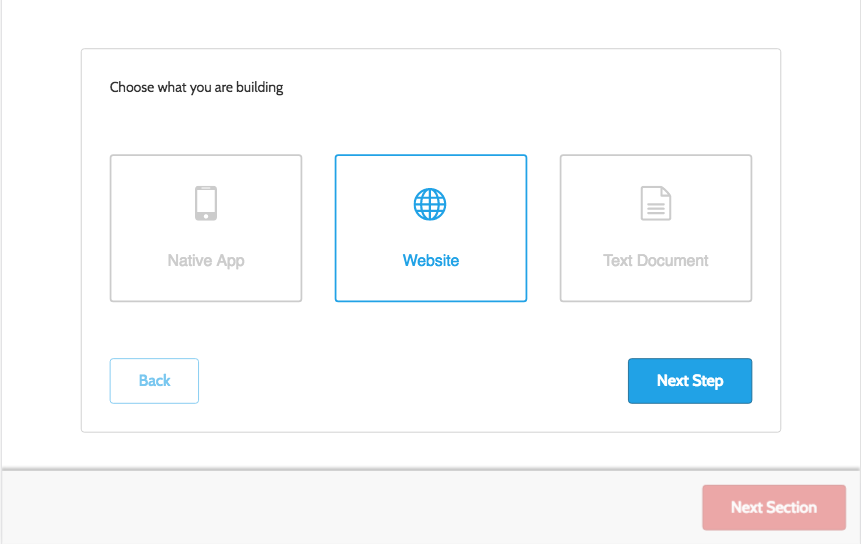
\includegraphics[width=1\textwidth]{images/25knots_entrance.png}
    \caption{Farben verschiedener interaktiver Elemente}
    \label{fig:entrance}
\end{figure}

Weiterhin gilt es zu beachten, dass der Nutzer die Anwendung verwendet, um eine Gestaltung für sein Projekt zu erstellen. Der Fokus der Anwendung sollte daher darauf liegen, dem Nutzer die von ihm erarbeitete Gestaltung zu zeigen. Die Anwendung sollte sich nur in bestimmten Fällen (beispielsweise beim Auftreten eines Fehlers oder wenn eine Interaktion notwendig ist) in den Vordergrund stellen. Daher wurde darauf geachtet, die Anwendung so simpel wie möglich zu gestalten und auf unnötige gestalterische Spielereien zu verzichten. Der größte Teil der Anwendung ist in Weiß- und Grautönen gehalten, um sie die Gestaltung des Nutzers und dessen Entscheidungen besser in den Vordergrund stellen zu können.

Dieses Vorgehen lässt sich anhand von zwei Beispielen gut verdeutlichen. Zum Einen seien hier die Fehlermeldungen im Bereich Typographie genannt. Diese sind in einem auffälligen Gelb hinterlegt, dass nur an dieser Stelle (im Sinne von: Zum anzeigen von Fehlern) verwendet wird und dem Nutzer dafür schnell auffällt (siehe Abbildung \ref{fig:warning}).
Zum Anderen zeig die Auswahl von Farben gut, wie Interaktive Elemente der Anwendung gleichzeitig auch die Gestaltung des Nutzer zeigen können. Die Buttons zur Auswahl einer Farbe (siehe Abbildung \ref{fig:accent}) bestehen hier lediglich aus der Farbe selbst, die Gestaltung der Anwendung wird hier als visuelle Zwischenebene also komplett entfernt.

\begin{figure}[h]
    \centering
    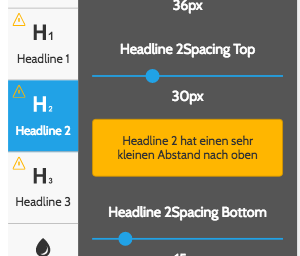
\includegraphics[width=0.5\textwidth]{images/25knots_Warning.png}
    \caption{Fehlermeldungen im Bereich Typographie}
    \label{fig:warning}
\end{figure}

\begin{figure}[h]
    \centering
    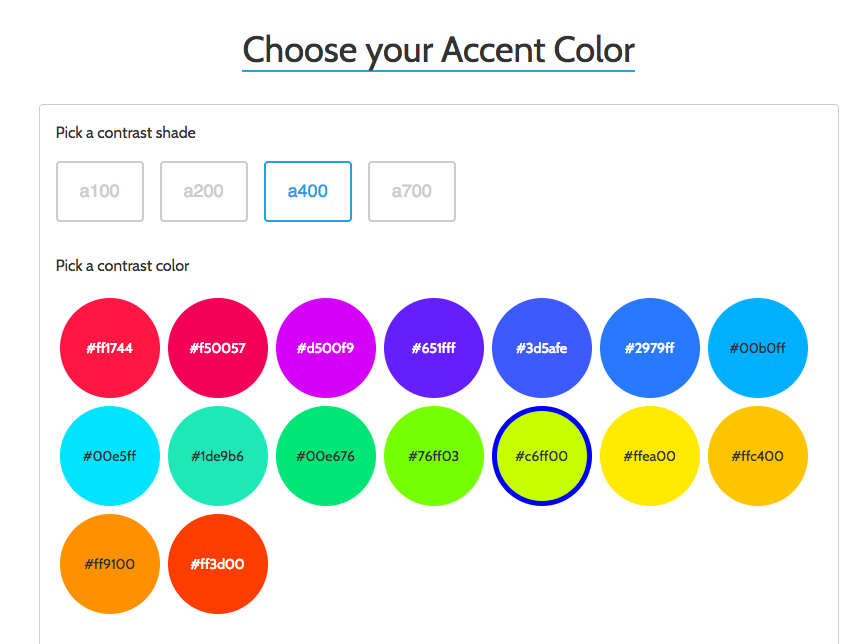
\includegraphics[width=1\textwidth]{images/25knots_color_button.png}
    \caption{Buttons zum Auswählen einer Akzentfarbe}
    \label{fig:accent}
\end{figure}


\subsection{Vorgehen}
Während der Gestaltung wurde sehr agil gearbeitet. Diese Agilität zeigt sich auf verschiedene Weise.
So waren der Entwicklungsprozess (gemeint ist hier die tatsächliche Programmierung) und der Gestaltungsprozess (das Entwickeln von MockUps in einem entsprechenden Programm) nicht strikt von einander getrennt, sondern überschnitten sich. Diese Überschneidung zeigt sich sowohl in einer Langfristigen betrachten, als auch in einer kurzfristigen. Es gab nicht einen Gestaltungsprozess, nach dessen Fertigstellung die Entwicklung startete, sondern vielmehr einen Gestaltungsprozess pro Schritt der Anwendung, der umgesetzt wurde. Auch innerhalb eines Schrittes war das Vorgehen nicht linear und es wurden häufig während der Entwicklung Aspekte in der Gestaltung verändert. Die Gründe hierfür sind vor allem eine bessere Möglichkeit zum testen der Interaktion während der Entwicklung.\\
Durch die in Kapitel \ref{chap:spacing} und \ref{chap:styleguide} erläuterten Aspekte konnten hier auch häufig kleinere Änderungen in der Gestaltung während der Entwicklung, ohne das Anpassen von MockUps, vorgenommen werden.

\subsection{Abstände}
\label{chap:spacing}
Um den Gedanken von innerhalb der Anwendung wiederverwendbaren Komponenten zu unterstützen liegt der Gedanke nahe, auch Abstände innerhalb der Gestaltung (und später auch in der Umsetzung) wiederverwendbar zu gestalten. Die Grundlage für diesen Gedanken lieferte ein Artikel von Nathan Curtis \cite{CurtisSpace16}. Der Artikel enthält zwei Grundgedanken:

\begin{enumerate}
  \item Die Größen von Abständen sollten sollten festgelegt und ihre Anzahl übersichtlich sein.
  \item Es gibt verschiedene Arten von Abständen, die die verschiedenen Größen auf unterschiedliche Weise einsetzen und kombinieren.
\end{enumerate}

Diese Gedanken wurden in der Gestaltung und Umsetzung des Projektes übernommen. Zunächst wurden die verschiedenen Abstände, aufbauend auf der von Curtis empfohlenen Basisgröße von 16px, definiert. Aufbauend auf der Basisgröße wurden anschließend Abstufungen in beide Richtungen
Erstellt, die nach Kleidergrößen, von XS bis XXL, benannt wurden.
Diese Abstufungen wurden in einer eigenen Datei als JavaScript-Objekt deklariert, so dass über die gesamte Anwendung hinweg diese festgelegten Größen verwendet werden können.

Curtis definiert 6 verschieden Arten von Abständen (vgl. Abb. ZXC), von denen 5 innerhalb der Anwendung als eigenständige Komponenten definiert wurden.
Die Komponenten nehmen die Größe des Abstandes als \verb|prop| in einer der definierten Kleidergrößen entgegen und erzeugen ein \verb|div|, dass die Abstände als padding oder margin anwendet.
Die Pixelwerte für die jeweilige Abstandsgröße erhält die Komponente dabei durch den Aufruf des für die Abstandsgrößen zuständigen JavaScript-Objekts (zum Beispiel \verb|spacing.l|). Alle diese Komponenten rendern außerdem die ihnen übergebenen Kinder, sodass eine Verwendung der \verb|SpacingInset| Komponente wie in Listing \ref{lst:spacingInset} möglich wird.

\begin{lstlisting}[caption=Beispielhafte Verwendung einer Komponente für Abstände, label=lst:spacingInset]
  <SpacingInset size='l' >
    <h1> A Headline </h1>
    <p> Some Text </p>
  </SpacingInset>
\end{lstlisting}

Hier stellt sich die Frage, inwiefern es Sinn ergibt, Komponenten zu definieren, die eine ausschließlich visuelle Funktion haben.
So könnte deren Funktion auch innerhalb der CSS-Regeln von anderen Komponenten definiert und so ein übersichtlicheres Markup geschaffen werden.
Während der Arbeit stellte sich heraus, dass die Definition er Abstände als eigene Komponenten ein sehr einfaches Entwickeln von Interfaces ermöglichte.  Durch die eingegrenzten Möglichkeiten ist auch währen der Entwicklung ein testen von anderen Abständen sehr einfach möglich.
Weiterhin ist der Raum für Inkonsistenzen begrenzt, da die Abstände nur in den vorgegebenen Größen angegeben werden können. Dies wurde, gerade mit Blick auf die spätere Weiterentwicklung und Veröffentlichung, als ausreichend großer Vorteil angesehen, um eine Definition als eigenständige Komponente zu rechtfertigen.

\subsection{Styleguide}
\label{chap:styleguide}
Da zu einem späteren Zeitpunk unter Umständen verschiedene Personen an der Weiterentwicklung der Anwendung beteiligt sein werden, macht das Festhalten der bisher gestalteten Elemente und der Grundlagen der Gestaltung durchaus Sinn.
Während der Gestaltung wurde nur ein minimalistischer Styleguide mit Informationen über Farben, Schriftgrößen und Abstände geführt, der für die Gestaltung dieser ersten Version mit nur einer Person im Team ausreichend war.

Mit Blick auf die spätere Weiterentwicklung durch ist ein Zentraler Ort, der einen Überblick über die bereits erstellten Komponenten gibt, von großem Vorteil.
Hierfür wurde die Bibliothek Storybook\footnotemark{} verwendet. Die Bibliothek läuft lokal im Browser und ermöglicht es, verschiedene Komponenten aus der Anwendung gekapselt darzustellen. Hierbei ist kein doppelter Code notwendig, die Komponenten können direkt aus dem Anwendungscode übernommen werden.
Das hat außerdem den Vorteil, dass Komponenten zunächst für sich, außerhalb der Anwendung und ohne mögliche Abhängigkeiten entwickelt werden können.

\footnotetext{\url{https://github.com/storybooks/storybook}}

\section{Architektur}
Bei der Textgestaltung und automatischen Änderung von Abbildungsnummern, Querverweisen,
Seitenzahlen, Gliederungen, Literaturhinweisen etc. bietet sich der Rückgriff
auf moderne Textverarbeitungsprogramme an. Nutzen Sie diese zur besseren Lesbarkeit
und Strukturierung des Textes, aber vermeiden Sie überflüssige Spielereien. Da
besonders bei Textdokumenten mit eingebundenen Objekten wie Bildern, Formeln

\subsection{Redux}
\label{chap:redux}

Im laufe der Anwendung müssen bestimmte Informationen üner die Gesamte Anwendung hinweg für bestimmte Komponenten abrufbar sein. Die betrifft vor allem, aber nicht ausschließelich die von Nutzer zu beginn der Interaktion mit der Anwendung definierten \textit{scopes}, die von jedem Teil der Anwendung für die korrekte Darstellung der angepassten Inhalte überprüft werden. Ein weiteres Beispiel stellt die zusammenfassung am Ende der Interaktion mit der Anwednung dar, die zugriff auf alle vom Nutzer definierten Werte benötigt. Der Redux-Store für die Anwendung umfasst daher Werte aus den Schritten \textit{Intro}, \textit{Typographie} und \textit{Farben}, die vollständige Struktur kann Listing ZXC entnommen werden.
Um die Arbeit mir dem Store zu simplifizieren und ein übermäßiges traversieren durch das Store-Objekt zu vermeiden, wurde für jeden der Bereiche ein dedizierter reducer geschrieben, der sich ausschließlich mit der Manipulation der diesem Schritt zugehörigen Werte befasst. In der Datei \verb|ApplicationState.js| werden diese mit Hilfe der Funktion \verb|combineReducers|, die von Redux zur Verfügung gestellt wird dann zu einem Objekt zusammengefügt (siehe Listing \ref{lst:combine_reducer}).

\begin{lstlisting}[caption={Zusammenfügen der dedizierten Reducer zu einem Objekt}, label=lst:combine_reducer]
  const ApplicationState = combineReducers({
    setup: setup,
    typography: typography,
    colors: colors
})
\end{lstlisting}

\subsubsection{Beispielhaftes Verändern des Redux Store}


\subsection{CSS-Architektur}
Für den Umgang mit CSS in React.js bieten sich verschiedene Möglichkeiten an. Nativ sind zwei Vorgehensweisen möglich: Anwenden von CSS über ausgelagerte Stylesheets (wie es in der Regel bei allen Webseiten gemacht wird) oder das verwenden von Inline-Styles.

Das verwenden von klassischen Stylesheets unterscheidet sich nicht sehr von der Verwendung bei einer statischen Webseite. Auch in React werden Klassennamen oder IDs festgelegt, über die dann im Stylesheet das Aussehen definiert wird (natürlich sind auch alle anderen validen CSS Selektoren anwendbar, Klassen und IDs seine hier nur als die populärsten Varianten beispielhaft genannt).
Auch die Verwendung von CSS-Präsporzessoren wie zum Beispiel SCSS stellt kein Problem dar, die kompilierung dieser Dateien muss lediglich in den Build-Prozess von React.js mit eingebunden werden. Eine simplifizierte Anwendung sähe beispielsweise wie folgt aus:

\begin{lstlisting}
<ReactComponent className='myClass'>
 Content
</ReactComponent>
\end{lstlisting}

Die kompilierte Dom-Node wäre dabei

\begin{lstlisting}
  <ReactComponent class='myClass'>
   Content
  </ReactComponent>
\end{lstlisting}

Und könnte im Stylesheet über

\begin{lstlisting}
  .myClass {
    color: red
  }
\end{lstlisting}

Angesprochen werden. Auch die Verwendung von Methodiken wie BEM oder SMACCS ist mit diesem Ansatz ohne Probleme möglich.
Für den Rahmen dieses Projektes wurde sich jedoch gegen diese Vorgehensweise entschieden, da bewusst ein Fokus auf eine komponentenbasierte Architektur gelegt werden sollte. Auch mit einer komponentenbasierten CSS-Architektur ist eine Komponente immer noch auf zwei Orte aufgeteilt: Die Funktion und das Markup, und das Styling.

[HIER LIESSE SICH AUCH DIE DISKUSSION NOCH AUSFÜHREN, DASS EIGENTLICH LEUTE LANGE DAFÜR GESPROCHEN HABEN, AUSSEHEN UND MARKUP ZU TRENNEN UND WARUM DAS HIER OKAY IST]

Um das Styling und die Funktion einer Komponente an einem Ort zu halten, bieten sich inline-styles an. Wie auch bei statischen Webseiten werden inline-styles direkt im \verb|style|-Attribut eines Elementes definiert. In React.js werden diese als JavaScript-Objekt übergeben. Eine Beispielhafte Anwendung findet sich in Quellcode XYZ

\begin{lstlisting}
  const styles = {
    backgroundColor: 'red',
    fontSize: '12px'
  }

  export default function myComponent(props) {
    return (
      <div styles=({styles}) >
  		{props.children}
  	  </div>
    )
  }
\end{lstlisting}

Auf den ersten Blick wirkt die Verwendung von inline-styles problematisch, vielleicht weil diese auf statischen Seiten viele Nachteile mit sich bringen. In einem Komponentenbasierten System wie React.js sind diese Nachteile jedoch nicht present. Durch die Komponentenbasierte Struktur und das damit einhergehende Ziel der Wiederverwendung von Komponenten, müssen Stylingänderungen auch hier nur an einer Stelle vorgenommen werden. Da jede Komponente nur für ihr eigenes Styling verantwortlich ist und nicht für das von Kindern, und auch kein CSS außerhalb der inline-styles verwendet wird (abgesehen von CSS-Reset und einigen globalen Regeln wie der Schriftart), kann es zu keinen Problemen mit der Spezifität von CSS-Regeln kommen.

Allerdings weisen inline-styles einige Limitierungen auf. So können beispielsweise keine Pseudo-Elemente wie \verb|:after| oder \verb|:before| verwendet werden. Auch das definieren von hover-states via \verb|:hover| wird nicht unterstützt.

[HIER NOCH VERWEIS AUF SPEZIFIKATION]

Zwar sind diese Limitierung zum aktuellen Stand des Projektes noch nicht von allzu großer Bedeutung, mit Blick auf eine Weiterentwicklung der Anwendung nach der Abschlussarbeit können diese in Zukunft jedoch eine größere Rolle spielen.
Um diese  Limitierungen zu umgehen, wurde das Framework Aphrodite verwendet. Das Framework erlaubt das Festlegen von styles innerhalb der Komponente ähnlich wie inline-styles, erzeugt aber für jedes neue style-objekt eine einzigartige CSS-Klasse, die via \verb|className| angewendet wird. Die Einzigartigkeit der Klasse wird durch das hinzufügen eines Hauses am Ende des Klassennamens gewährleistet.  Listing XYZ zeigt ein Beispiel

\begin{lstlisting}
  import React from 'react'
  import { StyleSheet, css } from 'aphrodite'

  function myComponent(props) {
  	<div className={css(styles.componentStyles)} >
  		{props.children}
  	</div>

  	const styles = StyleSheet.create({
  		componentStyles: {
  			color: 'blue'
  		}
  	})
  }
\end{lstlisting}

Die Struktur der style-objekte ist dabei der von inline-style-objekten gleich.

Mit der Verwendung von Aphrodite können also Aussehen und Funktion von Komponenten in der gleichen Datei gehalten werden, ohne dabei den Limitierungen von inline-styles zu unterliegen.


\section{Interessante Aspekte in der Entwicklung}

\subsection{State in Komponenten}
\label{chap:state_component}
Das Konzept des \textit{state} in React.js wurde Bereits in Kapitel \ref{chap:stateless} angesprochen. Hier soll an einem konkreten Bespiel verdeutlicht werden, wie der \textit{state} genutzt werden kann, um auf Nutzereingaben zu reagieren und an welcher Stelle sich der \textit{Component State} und der \textit{Application State} unterscheiden.
Als Beispiel wurde die Auswahl des Zielmediums durch den Nutzer im ersten Schritt der Anwendung gewählt, die in mehreren Schritten durchgeführt wird.
Der Ablauf der Interaktion mit der Anwendung sieht dabei wie folgt aus:
Die Anwendung präsentiert dem Nutzer drei Optionen, aus denen dieser wählen kann. Wählt der Nutzer eine der Optionen aus, gibt die Anwendung ihm eine visuelle Rückmeldung über die ausgewählte Option. Ist der Nutzer mit seiner Wahl zufrieden, bestätigt er diese durch einen Button und  ihm wir der nächste Schritt im Wizard angezeigt.

Für diese Interaktion werden verschiedene Komponenten eingesetzt (vgl. Abbildung ZXC), von denen die meisten \textit{stateless} sind, lediglich die Komponente \verb|SetupProgress|, die in Listing \ref{lst:setup} zu sehen ist\footnotemark{}, verwaltet einen Zustand.

\footnotetext{Teile des Quellcodes, die für diesen Anwendungsfall nicht relevant sind, wurden gekürzt. Die gesamte Datei kann der beiliegenden CD entnommen werden}

Im \textit{state} der Komponente \verb|SetupProgress| wird eine Zahl gespeichert die angibt, welche der angezeigten Optionen momentan aktiv ist (ist keine aktiv, wird der Wert auf \verb|false| gesetzt). Beim rendern der \verb|IconButton| Komponenten wird für jede Komponente abgeglichen, ob diese im \textit{state} als aktive Option gespeichert ist. Jede der \verb|IconButton|-Komponenten, die Angezeigt wird, ruft über einen Callback die Funktion \verb|handleIconButtonClick(key)| auf, wenn der User auf diese klickt und übergibt einen Key, der wiederum in den \textit{state} der  \verb|SetupProgress| Komponente geschrieben wird. Durch das aktualisieren des \textit{state} wird nun die \verb|render()| Funktion der Komponente erneut aufgerufen und die entsprechende \verb|IconButton| Komponente wird als aktiv markiert.
Der  \verb|IconButton| Komponente selbst ist dabei der Kontext, in dem sie verwendet wird, nicht bekannt.


\begin{lstlisting}[caption=Die Komponente \texttt{SetupProgress} in gekürzter Form, label=lst:setup]
  class SetupProgress extends React.Component {
    constructor(props) {
      super(props)

      // Shortened for readability

      this.state = {
        activeOption: false
      }
    }

    handleIconButtonClick(key) {
      this.setState({
        activeOption: key
      })
    }

    handleButtonClick() {
      this.props.setScope(this.state.activeOption)

      // If the current setup step is the last, also set the setup state to finished
      if (this.props.setupStep == this.props.setupSteps) {
        this.props.setSetupToFinished()
      }

      // Reset this components' internal state to disable the button
      this.setState({
        activeOption: false
      })
    }

    handleBackButtonClick() {
      this.props.previousSetupStep()
    }

    /**
     * Generates the main content for the setup component (i.e. Iconbuttons).
     * Determines the correct subset of options and calls constructIconButtons()
     * with that subset.
     *
     * @return {Array} An array of IconButtons ready for rendering
     */
    generateContent() {

      // Shortened for readability

      return this.constructIconButtons(setupOptions)
    }

    /**
     * Constructs an array of IconButtons based on a given set of options
     *
     * NOTE: This will construct an IconButton for every element in the given options
     * and does not validate them.
     *
     * @param {Array} setupOptions
     * @returns {Array} An Array of iconButtons
     */
    constructIconButtons(setupOptions) {
      let iconButtons = []
      for (var i = 0; i < setupOptions.length; i++) {
        let currentOption = setupOptions[i]

        iconButtons.push(
          <div className={css(styles.iconButtonWrapper)}>
            <IconButton
              icon={currentOption.icon}
              onClick={this.handleIconButtonClick}
              key={i}
              identifier={currentOption.value}
              active={this.state.activeOption === currentOption.value}
            >
              {currentOption.text}
            </IconButton>
          </div>

        )
      }

      return iconButtons
    }

    render() {
      return (
        <BorderedBox>
          <SpacingInset size='l'>
            <span>Choose what you are building</span>
            <SpacingInset size='l' />
            <div className={css(styles.buttonWrapperStyles)}>
              {this.generateContent()}
            </div>
            <SpacingInset size='l' />
            <div className={css(styles.buttonWrapperStyles)}>
              <SecondaryButton inactive={this.props.setupStep < 2} onClick={this.handleBackButtonClick} variant={'outline'}>Back</SecondaryButton>
              <SecondaryButton inactive={this.state.activeOption == false} onClick={this.handleButtonClick}>Next Step</SecondaryButton>
            </div>
          </SpacingInset>
        </BorderedBox>
      )
    }
  }

  // Shortened for readability

  export default SetupProgress
\end{lstlisting}

Der hier gezeigte Ablauf hätte sich auch durch die Verwendung des Redux-Stores realisieren lassen, jedoch ist die gewählte Option zunächst nicht für die gesamte Anwendung von Relevanz (so kann der Nutzer seine Auswahl zum Beispiel noch ändern). Erst, wenn der Nutzer sich durch den Klick auf den \textit{Next}-Button auf einen Wert festlegt, wird dieser auch der ganzen Anwendung, über den Redux-Store, bekannt gemacht.

\subsection{Dispatch von Actions}
Das Hauptaugenmerk in der Entwicklung lag in diesem Schritt im setzen der Scopes für die Anwendung. Da auf die Scopes in allen späteren Teilen der Anwendung zugegriffen werden können muss wurde schnell deutlich, dass diese im Application Sate, also dem Redux Store gehalten werden müssen. Hier stellte sich jedoch vor allem die Fragen nach der Datenstruktur der Scopes, wobei die Möglichkeiten auf die Haltung in einem Array oder als JavaScript Objekt begrenzt wurden.
Ein Array bietet dabei eine höhere Flexibilität, jedoch eine deutlich ungenauere Beschreibung der Scopes. So können andere Komponenten herausfinden, ob der für ihren Anwendungsfall relevanten Scope sich im Array der Scopes befindet, ohne Kenntnis darüber haben zu müssen, wie der Schlüssel des Scopes innerhalb des JavaScript Objektes lautet. Auch spielt die Länger der verschiedenen Äste des Baumes bei der Verwendung des Arrays eine weniger große Rolle, während bei der Verwendung eines Objektes immer auch geprüft werden muss, ob der key im store überhaupt vorhanden ist. Daher wurde an dieser Stelle ein Array verwendet.
[HIER SPÄTER NOCH MAL SCHAUEN, OB DAS NOCH STIMMT]

\subsection{Anzeige von Inhalten nach Scope}
Ein Hauptaugenmerk währen der Entwicklung lag auf der Anwendung der vom Nutzer gewählten \textit{scope} in der Anwendung. In Abhängigkeit dieser Scopes muss die Anwendung verschiedene Daten präsentieren. Dabei muss die Möglichkeit bestehen, diese Daten zu erweitern oder zu verändern, ohne dass die Anwendung selbst dafür umstrukturiert werden muss. Diese Datenhaltung soll hier am Beispiel der verschiedenen Schriftfamilien, die im Bereich Typographie Verwendung finden können, gezeigt werden.

Da die Anwendung keine Datenbank implementiert, werden diese Daten in eigenen Dateien als JavaScript-Objekte gespeichert. Listing \ref{lst:fonts_object} zeigt das Objekt, in dem die verschiedenen Schriftarten der \textit{scopes} als Arrays gespeichert sind. Bei Betrachtung des Objektes fällt auf, dass sich Daten teilweise wiederholen. Obwohl hier gegen das Prinzip \textit{Don’t Repeat Yourself} verstoßen wird, ist eine solche Struktur mit Blick auf eine Weiterentwicklung der Anwendung nötig, um ein möglichst einfaches Verändern eines einzelnen \textit{scopes} gewährleisten zu können.

\begin{lstlisting}[caption=Aufbau des \texttt{FONTS} Objektes, label=lst:fonts_object]
  export const FONTS = {
    DISPLAY: [
      'Verdana', 'Arial', 'Tahoma', 'TrebuchetMS'
    ],
    RESPONSIVE: [
      'Verdana', 'Arial', 'Tahoma', 'TrebuchetMS'
    ],
    NOT_RESPONSIVE: [
      'Verdana', 'Arial', 'Tahoma', 'TrebuchetMS'
    ],
    PAPER_DISPLAY: [
      'Verdana', 'Arial', 'Tahoma', 'TrebuchetMS', 'Times New Roman', 'Georgia', 'Palatino'
    ],
    PAPER: [
      'Times New Roman', 'Georgia', 'Palatino'
    ],
    ANDROID: [
      'Roboto', 'Noto'
    ],
    IOS: [
      'San Francisco'
    ]
  }
\end{lstlisting}

Da die \textit{keys} im \verb|FONTS| Objekt dabei exakt den möglichen \textit{scopes} entsprechen\footnotemark{}, ist ein einfaches Ermitteln der benötigten Schriftfamilien, wie es in Listing \ref{lst:fonts_access} gezeigt wird, möglich.

\footnotetext{Auch die verschiedenen \textit{scopes} sind Konstanten, die in einem Objekt gespeichert werden.}

\begin{lstlisting}[caption=Zugriff auf Werte des \texttt{FONTS} Objektes, label=lst:fonts_access]
  determineFontFamilies() {
    let scope = this.props.scopes[1]
    return FONTS[scope]
  }
\end{lstlisting}


\subsection{Modularisierung der Anwendung}
\textbf{Hier ist gemeint: Im Praxisprojekt wurden mehr Komponenten gebraucht, was lief hier besser?}
Im Vergleich zum Praxisprojekt wurde weiterhin der Komponentenbasierte Aufbau verbessert. Währen im Praxisprojekt noch 21 Komponenten für die Darstellung verwendet wurden, konnte diese Zahl im rahmen der Abschlussarbeit auch 10 verringert werden.\\
\textbf{[ WIE KONNTE DAS ERREICHT WERDEN? ]}

Dies lässt sich beispielhaft an der Komponente aufzeigen, die verschiedene Möglichkeiten zur Manipulation von Attributen von Überschriften darstellt. In der Anwendung gibt es drei Überschriften verschiedener Ordnung, die in den Werten Größe,  Abstand nach oben und Abstand  nach unten verändert werden können. Im Praxisprojekt gab es hier für jede Überschrift verschiedener Ordnung eine eigene Komponente, im Rahmen der Abschlussarbeit konnte dies auf nur eine Komponente reduziert werden.\\
Der Hauptgrund hierfür ist das auslagern der Logik in andere Bereiche der Anwendung. So werden die Fehler nicht mehr innerhalb der Komponente errechnet, sondern lediglich dargestellt. Alle anderen Werte werden der Komponente beim Aufruf aus der Elternkomponente übergeben. Die prop area gibt dabei an, welchen Bereich des Stores diese Komponente verändert.

\begin{lstlisting}
  <HeadlineControls
  	onChange={this.props.setValueInArea}
  	area={'headline1'}
  	title={'Headline 1'}
  	componentErrors={errors.headline1}
  	{...this.props.headline1}
  />
\end{lstlisting}

\subsection{Erstellen von Farbkontrasten}
Die Grundlegende Logik zum errechnen von bestimmten Kontrasten wurde bereits im Praxisprojekt definiert. Im ersten Schritt muss die Grundfarbe hierfür in den HSL-Farbraum überführt werden. Für diese Umwandlung wurde in der Anwendung die Bibliothek tinycolor\footnotemark{} verwendet, die verschiedene Funktionen zur Arbeit mit Farben bereit stellt (unter anderem auch das Umwandeln in den HSL-Farbraum).
Nach der Umwandlung in den HSL-Farbraum gibt die Bibliothek ein JavaScript-Objekt zurück, in dem \textit{Hue}, \textit{Saturation}, \textit{Lightness} und \textit{Alpha} als \textit{Key-Value}-Paare vorhanden sind, mit denen die Berechnungen für die Farbkontraste vorgenommen werden können.

\footnotetext{\url{https://github.com/bgrins/TinyColor}, zuletzt abgerufen am 10.8.2017}

Für einen Komplementär-Kontrast muss der \textit{Hue}-Wert der Grundfarbe um 180° verändert werden. Die Berechnung erwies sich mit Hilfe des HSL-JavaScript-Objektes als recht simpel, hier musste lediglich darauf geachtet werden, den einen Wert von 360 nicht zu überschreiten. Listing \ref{lst:complementary} zeigt die Funktion \verb|calculateComplemntary|, die diese Berechnung ausführt.

\begin{lstlisting}[caption=Berechnung eines Komplementär-Kontrastes, label=lst:complementary]
  export function calculateComplemntary(baseColor) {
    let complementary = Object.assign({}, baseColor)
    let hue = complementary.h

    hue += 180
    if (hue > 360) {
      hue -= 360
    }

    complementary.h = hue
    return complementary
  }
\end{lstlisting}

Hier wurde außerdem darauf geachtet, das Farbobjekt mit Hilfe der Funktion \verb|Object.assign()| zu kopieren, um keine ungewünschten Veränderungen im \verb|baseColor|-Objekt zu erzeugen\footnotemark{}.

\footnotetext{Objekte in JavaScript werden als \textit{Referenz} übergeben, siehe dazu \cite{Aggarwal2017Explaining}}

Die Berechnung des triadischen Kontrastes gestaltet sich ähnlich, Hier wurde der \textit{Hue}-Wert jedoch um 30° erhöht beziehungsweise verringert, um den gewünschten Effekt zu erzielen.

Deutlich komplexer gestaltet die Generierung von monochromatischen Farbschemata, da die Farben hier in ihrem \textit{Hue}-Wert unverändert bleiben, jedoch in ihrem \textit{Saturation} und/oder ihrem \textit{Lightness}-Wert verändert werden können. Weiterhin werden für dies Farbschema mehr Farben benötigt (die Anwendung arbeitet mit der Grundfarbe und drei weitern, veränderten Farben).

Für jede Farbe müssen hier also verschiedene Entscheidungen getroffen werden. Zunächst muss entscheiden werden, welche Werte verändert werden können. Möglich ist hier einer von drei Fällen:

\begin{itemize}
  \item Nur der \textit{Saturation}-Wert
  \item Nur der \textit{Lightness}-Wert
  \item Sowohl der \textit{Saturation}- als auch der \textit{Lightness}-Wert
\end{itemize}

Um hier dynamischere Ergebnisse liefern zu können, wird diese Entscheidung in der Funktion \verb|calculateMonochromaticColors|, die Listing \ref{lst:mono} zeigt, zufällig getroffen.

\begin{lstlisting}[caption=Berechnung eines Monochromatischen Farbschemas, label=lst:mono]
  calculateMonochromaticColors(amount) {

    let colors = []

    for (var i = 0; i < amount; i++) {
      let currentColor = Object.assign({}, convertToHsl(this.props.baseColor))
      // Figure out if only one or two values should be changed
      // Random: 0 = Lightness, 1 = Saturation, 2 = Both
      let randomOption = Math.floor(Math.random() * 3)
      let changedColor = this.changeValuesOfColor(randomOption, currentColor)

      if (colors.length < 1) {
        colors.push(changedColor)
      } else {
        let similarColors = this.checkForSimilarColors(colors, changedColor)
        while (similarColors) {
          changedColor = this.changeValuesOfColor(randomOption, changedColor)
          similarColors = this.checkForSimilarColors(colors, changedColor)
        }
        colors.push(changedColor)
      }
    }

    return colors
  }
\end{lstlisting}

Im nächsten Schritt müssen die Veränderungen in den bestimmten Werten vorgenommen werden. Auch hier werden diese Werte zufällig gewählt, wobei die Farben nicht zu Dunkel oder zu hell sein dürfen. Diese Zuweisung findet in der Funktion \verb|changeValuesOfColor| statt (siehe Listing \ref{lst:hsl}).

[ HIER NOCH ERKLÄREN, WIE HELLE UND DUNKLE FARBEN AUSGESCHLOSSEN WERDEN ]

\begin{lstlisting}[caption=Setzen der HSL-Werte, label=lst:hsl]
  changeValuesOfColor(values, color) {
    let manipulatedColor = Object.assign({}, color)
    // Switch case
    // Do the changes that need to be DropdownController
    switch (values) {
      case 0:
        // change lightness
        manipulatedColor.l = Math.random().toFixed(2)
        break
      case 1:
        // change Saturation
        manipulatedColor.s = Math.random().toFixed(2)
        break
      case 2:
        // change lightning and saturation
        manipulatedColor.l = Math.random().toFixed(2)
        manipulatedColor.s = Math.random().toFixed(2)
        break
      default:
        throw new 'Oops, seems like the randomizer messed something up.'
    }

    return manipulatedColor
  }
\end{lstlisting}

Nachdem die Farben festgelegt sind muss außerdem überprüft werden, ob  eine generierte Farbe a) zu ähnlich der Grundfarbe oder b) zu ähnlich einer anderen generierten Farbe ist.
Als \textit{zu ähnlich} zueinander wurden hier zwei Farben definiert, der \textit{Saturation}- \textbf{und} \textit{Lightness}-Werte eine Differenz kleiner als 0.1 aufweisen. Farben, die nur in einem der Beiden Werte eine zu kleine Differenz aufweisen, werden nicht als \textit{zu ähnlich} verstanden.
Die Ähnlichkeit zweier Farben wird in  der Funktion \verb|checkForSimilarColors| in Listing \ref{lst:similar} deutlich. Die Funktion gibt dabei \verb|true| zurück, wenn die beiden übergebenen Werte zu ähnlich sind. Anstatt der betroffenen Farbe wird dann eine neue generiert.

\begin{lstlisting}[caption=Überprüfen der Ähnlichkeit zweier Farben, label=lst:similar]
  checkForSimilarColors(colors, candidate) {
    let similarValues = false
    for (var j = 0; j < colors.length; j++) {
      let saturationDifference = Math.abs(colors[j].s - candidate.s)
      let lightnessDifference = Math.abs(colors[j].l - candidate.l)

      if (saturationDifference < 0.1 && lightnessDifference < 0.1) {
        similarValues = true
      }
    }

    return similarValues
  }
\end{lstlisting}


\subsection{Erstellen von PDF-Dateien}
Wie im Kapitel 2.1.2 “Ergebnisse der Benutzung”  bereits angesprochen, dient dieser letzte Schritt der Anwendung dazu, dem Nutzer eine Zusammenfassung der Ergebnisse zu liefern.
Da alle vom Nutzer getroffenen Entscheidungen im redux store gespeichert werden ist es kein Problem, hier eine Zusammenfassung dieser Daten darzustellen.
Diese Daten werden dem Nutzer in der aktuellen Version nach Themengebiet aufgeschlüsselt, untereinander dargestellt. Für die aktuell implementierten Gebiete und die daraus resultierende Menge an Informationen ist diese Lösung ausreichend, jedoch muss mit weiterer Entwicklung der Anwendung hier vermutlich auch ein anderer Lösungsansatz gefunden werden.

Als Anspruchsvoller stellte sich die Implementierung der Möglichkeit heraus, die Ergebnisse auch als PDF-Datei speichern zu können. Hier bieten sich verschiedene Möglichkeiten der PDF-Generierung an. Da die Applikation momentan eine reine Client-Anwendung ist, war die Auswahl an Möglichkeiten dadurch limitiert. Hier sollte nicht nur für die Möglichkeit der PDF-Generierung auch ein Server in die Anwendung eingespielt werden.

Die simpelste der Möglichkeiten ist ein Drucken als PDF Datei. Hierbei müsste für die Seite lediglich ein entsprechendes Stylesheet hinterlegt werden, dass das Layout für den Druck anpasst. Diese Lösung ist allerdings nur beschränkt verfügbar. Das Betriebssystem macOS bieten den Druck als PDF nativ an, das Betriebssystem Windows beispielsweise aber erst seit der neusten Version, Windows 10.
Eine weitere Möglichkeit stellt die Bibliothek html2canvas\footnotemark{} dar. Die Bibliothek erlaubt das Speichern von Seiten als Bilddateien. Die Verfügbarkeit ist hier deutlich höher als beim Drucken als PDF, jedoch bringt das Speichern als Bild einige Restriktionen mit sich. So können beispielsweise Werte nicht markiert und kopiert werden, was einen erhöhten Arbeitsaufwand für den Nutzer bedeutet.

\footnotetext{\url{https://github.com/niklasvh/html2canvas}}

Die Entscheidung file aus diesen Gründen hier auf die Bibliothek jsPDF\footnotemark{}. Diese erlaubt das erstellen von PDF-Dateien im Browser und auch das einfügen von DOM-Elementen in PDF-Dateien. Das einfügen bringt allerdings einige Limitierungen mit sich, so werden teilweise Texte, die zu tief in DOM-Elementen verschachtelt sind, nicht dargestellt. Daher wurde die PDF per hand zusammen gesetzt. jsPDF bietet dafür eine API, mit der verschiedene Elemente (wie Text oder geometrische Formen), unter Angabe der Position auf der x- und y-Achse, in die Datei eingefügt werden können. Listing XZY zeigt das beispielhafte einfügen einer Textzeile und das anschließende Speichern der Datei.

\footnotetext{\url{https://github.com/MrRio/jsPDF}}

Hier besteht jedoch ein hoher manueller Aufwand, der mit potentiellen weiteren Themengebieten in der Anwendung erneut evaluiert werden muss. Abb. XZY zeigt eine beispielhafte PDF-Datei, die von der Anwendung erstellt wurde.

Hier wurde außerdem deutlich, dass eine mögliche Nomenklatur des Projektes durch den Nutzer Vorteile hätte. So könnte dieser Name auf der PDF-Datei vermerkt werden, um diese eindeutiger zuordnen zu können. Außerdem wird dem Nutzer somit eher das Gefühl vermittelt, dass er einen Prozess durchläuft, an dessen Ende er ein Ergebnis für sein Projekt erzielt hat.
